\documentclass[runningheads]{llncs}
\usepackage{tikz}
\usetikzlibrary{bayesnet}
\usepackage{amsmath}
\usepackage{amsfonts}
\usepackage{rotating}
\usepackage{graphicx}
\usepackage{subfigure}
\usepackage{tikz}
\usepackage{multirow}
\usepackage[linesnumbered,boxed]{algorithm2e}
\usepackage{cite}
\setlength{\abovecaptionskip}{10pt}
\setlength{\belowcaptionskip}{-10pt}
\newcommand{\Ep}{\mathbb{E}}
\newcommand{\Real}{\mathcal{R}}
\newcommand{\Gaussian}{\mathcal{N}}
\usepackage{graphicx}


\begin{document}
%title change
\title{Model Sentiment Evolution For Social Incidents}

\author{Submission }
%anonymous
%\author{Yunjie Wang\inst{1} \and Xiaoli Wang\inst{1}\and Lin Sun\inst{2} \and Chen Lin\inst{1}}
%\authorrunning{Y.Wang et al.}
%\institute{Department of Computer Science, Xiamen University, China \email{chenlin@xmu.edu.cn} \and NatureWake Network Technology Co.,Ltd}

\maketitle             

\begin{abstract}
Modeling sentiment evolution for social incidents in microblogs is of vital importance for both researchers and government officials. 
Existing work on sentiment tracking is not satisfying, due to the lack of entity-level sentiment extraction and accurate sentiment shift detection.  
Identifying entity-level sentiment is challenging as microbloggers often use multiple opinion expressions in a sentence which targets towards different entities.
To address this problem, in this paper, we investigate the impact of proximity information to obtain more precise entity-level sentiment extraction.
Furthermore,detecting sentimen shift is not a trivial problem because the evolution of the background sentiment can not be ignored. 
We propose to simutanously model the evolution of sentiment and sentiment shift by a state space model on the time series of sentiment polarities.
Experiments on a real data set demonstrates that the proposed methods outperform state-of-the-art methods.
\keywords{Sentiment Tracking  \and Dynamic Sentiment Model \and Opinion Analysis \and Microblog Mining }
\end{abstract}

\section{Introduction}
%Motivation
Nowadays Microblogging has become the major platform for Chinese people to publish information and share opinions about social incidents. Public opinion on Microblogging platforms has greatly influenced the Chinese society, for some incidents even change the investigation and judicial outcome~\cite{{Cheung2014Battle}}. 
For example,  %change 
The power of public opinion in Microblogging space makes it appealing to analyze sentiment evolution for social incidents in microblogs for individuals, enterprises, NGO organizations, researchers, and government officials and so on.

%Problem studied
In this paper, to facilitate understanding of public opinions, we focus on the problem of modeling sentiment evolution for social incidents. 
Given a sequence of microblogging comments related to any social incident, our goal is to reveal the sentiment evolution pattern related to the involved entities in this incident and identify the significant sentiment shifts. 
As shown in Fig.~\ref{fig:tweet}, analysis of online comments on the murdur case of Jiang Ge\footnote{The murdur case of Jiang Ge, a Chinese student killed in Japan in 2016 has attracted wide attention online. Jiang was stabbed to death in her appartment by her rommate's boyfriend. After the tragegy, Jiang's mother (Jiang) blamed her daughter's roomate (Liu) for her daughter's death by claiming Liu had locked Jiang out when she was attacked.} leads to visualization of the evolution pattern of public sentiment towards the victim's mother (Jiang) and the victim's roomate (Liu). A sentiment shift is also detected in the third time point. %more specific, better describe the incident first

%first layer: input sequence from left to right, balanced text size
%input: background tweets in each time slice 1~2
%second layer output entity-specific sentiment polarity +- bar graph , aim to visualize evolution
%third layer  entity specific vocabulary
%forth layer shift, background tweet 

\begin{figure}
    \centering
    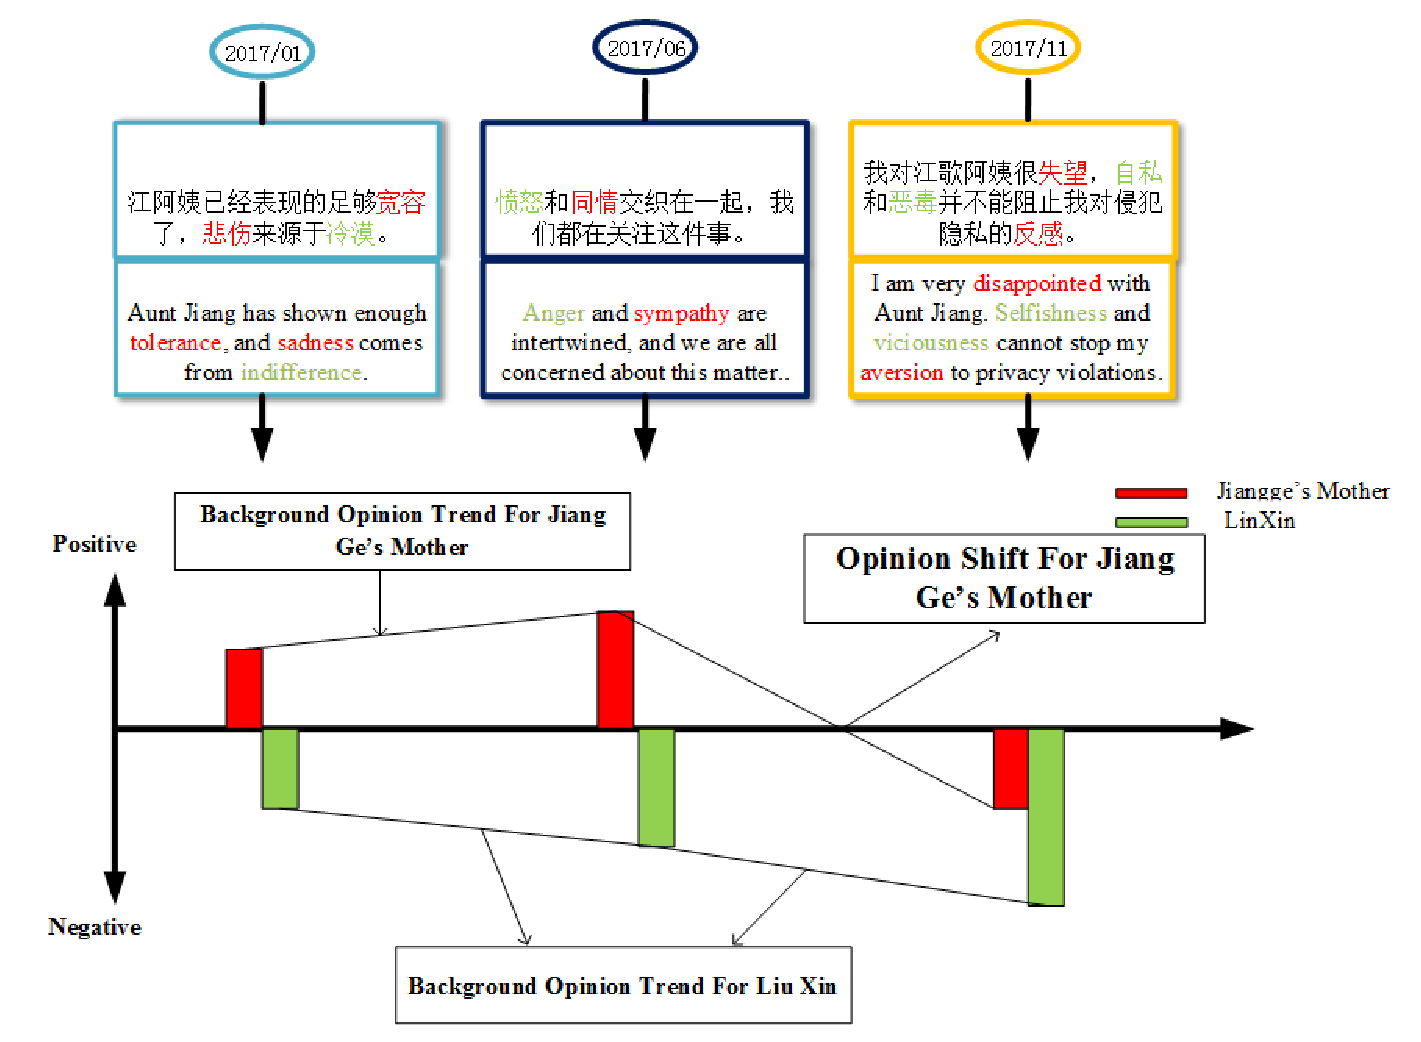
\includegraphics[width=1.0\textwidth,height=3.5in]{tweet.eps}
    \setlength{\abovecaptionskip}{-0.1cm}
    \caption{Comments from ``Jiang Ge'' incident and reflected characteristics of social incident.}\label{fig:tweet}
\end{figure}

%Related work
Recently there is an increasing interest in tracking microblogging sentiments for entities~\cite{Giachanou2016sentichange,Giachanou2017sentichange} or topics~\cite{Tsytsarau2014Topics,Thelwall2011topic}. Most of them are based on a two stage framework, i.e. first adopt a sentiment extraction tool such as SentiStrength~\cite{sentistrength2010} to compute the sentiment score for an entity or topic, then conduct statistical analysis such as outlier detection to obtain sentiment spikes. However, modeling public opinion for social incidents poses two challenges that haven't been addressed by previous research.

%mixed feelings
The first challenge is to \textbf{identify entity-level sentiment}. 
As a social incident often involves several entities (i.e. people or organizations), it is clearly problematic to utilize coarse-grained analysis which obtains an averaged sentiment for an event without separating different entities. %second layer
However, extracting entity level sentiment is not a trivial problem because the length limit of microblogs encourage people to use short and informal expressions.
Multiple opinion expressions are put in a sentence which targets towards different entities.
For example, as shown in Fig.~\ref{fig:tweet}, sentiment words for Jiang (in red) and for Liu (in green) are mixed together without a clear partition and a correct grammar structure. 
To address this challenge, it is helpful to \textbf{embed proximity information} to enhance entity-level sentiment extraction accuracy. 



%background evolution + shift
The second challenge is to \textbf{detect sentiment shift}.
In previous work, researchers mostly depend on statistical analysis such as outlier detection to detect sentiment spikes~\cite{Giachanou2016sentichange,Giachanou2017sentichange,Giachanou2016sentitime}.
Such a method is not sufficient, because the evolution of the background is largely overlooked.
The fact that events are continuously changing causes changing responses in public opinions. Hence sentiment shift should be distinguished with the evolution patterns of background sentiment.  
For example, in Figure~\ref{fig:tweet}, the background sentiment towards Jiang is an increasing trend of positive sentiment. Revealing this evolution pattern marks the significance of sentiment shift at the third time point. %running example
In this article we propose a probabilistic model that \textbf{simultaneously model the evolution of background opinion and the opinion shifts}.

%contributions
Our contributions are two folds. 
\textbf{In the application aspect}, we explore the feasibility of tracking sentiment evolution for social incidents on Chinese microblogs. Our work sheds insights into better understanding public opinions and provides a solid foundation for future applications such as explaining the causes of sentiment shifts. 
\textbf{In the model aspect}, we propose to simutanously model the evolution of background sentiment and sentiment shift by state space models on the natural parameters of the binomial distributions that represent the sentiment polarity. 
Furthermore, we investigate the impact of proximity information in obtaining entity-level sentiment extraction.


This paper is organized as follows. We briefly survey the related work in Sec.~\ref{sec:related}. In Sec.~\ref{sec:sentiment classification} to Sec.~\ref{sec:public opinion model}, we describe the methodology. We present and analyze the experimental results on a real data set in Sec.~\ref{sec:Experiment}. We conclude our work and suggest future directions in Sec.~\ref{sec:conclusion}.


\section{Related Work}\label{sec:related}
%sentiment tracking
\textbf{Sentiment Tracking on Microblogs} has received considerable attention from both academy and industry~\cite{Giachanou2016sentichange,Giachanou2017sentichange,Giachanou2016sentitime,An2014sentimentchange,Bollen2011sentimentchange,Tan2014topic,Montero2016sentimentchange}. Most of existing work adopt a cascade framework, i.e. in the first step sentiment of each tweet is extracted, in the second step sentiment shift is detected~\cite{Giachanou2016sentichange,Giachanou2017sentichange,Giachanou2016sentitime,An2014sentimentchange,Bollen2011sentimentchange,Tan2014topic}. To extract sentiment, the collection of tweets are divided into numerous time slices, and the ratio of positive and negatie sentiments is computed in a time slice~\cite{Giachanou2017sentichange,Giachanou2016sentitime,An2014sentimentchange,Bollen2011sentimentchange}. 
To detect sentiment shift, residual between actuarial and predicted sentiment value is the most commonly adopted measurment~\cite{Giachanou2016sentichange,Giachanou2016sentitime}. 
Furthermore, topic information is incorporated in recent studies. Sentiment change is represented by topic changes in~\cite{Tan2014topic}, an integrate framework based on empirical heuristics is utilized in~\cite{Montero2016sentimentchange} to identify
the emotional spikes and locate causes of spikes.%integration 

%sentiment analysis
A fundamental block in sentiment tracking systems is \textbf{sentiment analysis}. In the literature, there are two types of sentiment analysis algorithms: supervised learning and lexicon-based methods~\cite{Ahmed2017SentiCR}. \textbf{Supervised learning method} creates a training model based on training data
to classify the sentiment polarity of sentences. Obtaining training data and selecting features are the two most important parts of this methods. 
Emoji is often used to label sentiments of tweets~\cite{Go2009Supervisedlearning,Pak2010Supervisedlearning}. Hashtag is another major source to label training data~\cite{Papadopoulos2012SocialEvent}.
But the accuracy of label by emoji is low. To overcome this issue, an ensemble of sentiment detection tools is employed to obtain the training data~\cite{Barbosa2010Supervisedlearning}. 
The goal of supervision based methods is to classify the polarity of sentiments. To obtain a high precision, lexical features such asu nigrams and POS~\cite{Go2009Supervisedlearning,Davidov2010Supervisedlearning}, syntax features  such as  retweets, URLs, emoticons, and meta-features such as  POS tags, words’ polarity,~\cite{Barbosa2010Supervisedlearning} are obtained.
Experiments have shown that classifiers benefit most from features which involve text polarity~\cite{Agarwal2010Supervisedlearning}.

Due to the lack of training data, most researchers turn to \textbf{lexicon based methods}. 
SentiStrength is the first open domain large-scale lexicon, which is used as a baseline in most sentiment detection algorithms like SentiStrength2~\cite{Thelwall2012lexicon}, SentiStrength-SE~\cite{Rakibul2017SentiStrength-SE}, and VADER~\cite{Hutto2014SSimproved}. 
SentiSterength2~\cite{Thelwall2012lexicon} improves the accuracy of SentiStrength by adding idioms. 
VADER~\cite{Hutto2014SSimproved} improves the accuracy of SentiStrength by grouping sentiment words on Twitter and manually filtering them. 
SenciStrength-SE improves the recall of SentiStrength by designing different lexicons for different domains~\cite{Rakibul2017SentiStrength-SE}. 
The above methods are based on static lexicons.
Recently,we've seen an emerging attempt to construct dynamic lexicon. 
For example, to enclose subtle dimensions of a word’s sentiment, a seed lexicon is defined in ~\cite{Feng2011lexicon} and connotation lexicon is retrieved based on PageRank and HITS. 
%However, such a connotation lexicon is still noisy and often not scalable, because it contains sentiment words that are not related to any entity in an event.
However, directly applying these lexicons does not guarantee the accuracy of entity level sentiment extraction, because opinion expressions towards different entities are usually mixed toghether in a microblogging post. 


\section{Proximity-based Entity-level Sentiment Extraction}\label{sec:sentiment classification}
%problem definition? input output? preliminaries
In this section, we describe Proximity-based Entity-level Sentiment Extraction (PESE). Given xxx, our aim is to xxx.

\subsection{Distance Function}
%assumption
Our basic assumption is that the position of a sentiment word influences the performance of sentiment extraction. Intuitively, the closer a sentiment word is to an entity, the more likely the sentiment word is to describe the entity. Inspired by~\cite{}, we use four distance kernel functions to compute influence of sentiment words on entities, namely Gaussian, Triangle, Cosine, and Circle:

\textbf{1. Gaussian kernel}
\begin{equation}
    k(i,j) = \exp\left[\frac{-(i-j)^2}{2\sigma^2}\right],
\end{equation}

\textbf{2. Triangle kernel}
\begin{equation}
k(i,j)=\begin{cases}
1-\frac{|i-j|}{\sigma} &\mbox{if $|i-j|\leq \sigma$}\\
0 &\mbox{otherwise},
\end{cases}
\end{equation}

\textbf{3. Cosine (Hamming) kernel}
\begin{equation}
k(i,j)=\begin{cases}
\frac{1}{2}\left[1+cos\left(\frac{|i-j|\cdot\pi}{\sigma}\right)\right] &\mbox{if $|i-j|\leq \sigma$}\\
0 &\mbox{otherwise},
\end{cases}
\end{equation}

\textbf{4. Circle kernel}
\begin{equation}
k(i,j)=\begin{cases}
\sqrt{1-\left(\frac{|i-j|^2}{\sigma}\right)} &\mbox{if $|i-j|\leq \sigma$}\\
0 &\mbox{otherwise},
\end{cases}
\end{equation}

where $i$ is the position of the sentiment word in the sentence, and $j$ is the position of the entity in the sentence. All four of these kernel functions are governed by one parameter $\sigma$, which is tunned in the experiment.

We use the average of all sentiment words on the entity as the sentiment polarity of the sentence.

\subsection{Calculate Entity level Sentiment polarity}
To calculate the sentiment value for an entity given a post, we first calculate the influence of each sentiment words on the entity:
\begin{equation}\label{equ:influence}
    s_i = (-1)^n\cdot d_i\cdot v_i\cdot k(p_i,j),
\end{equation}
where $i$ is the number of this sentiment word. $n$ is the number of gainsay words between this sentiment word and the sentiment word before it. $d_i$ is the sum of the weights of the degree words between this sentiment word and the sentiment word before it. $v_i$ is the sentiment value of this sentiment word. $k$ is the distance function. $p_i$ is the location of this sentiment word. $j$ is the location of the entity.%????

We calculate the influence of all sentiment words on the entity according to Equ.~\ref{equ:influence}, and take the average value as the sentiment value of the sentence. If the sentiment value is greater than 0, we think that the sentence has a positive emotion. If the sentiment value is less than 0, we think that the entity has a negative emotion.



\section{Public Opinion Model}\label{sec:public opinion model}
%problem definition, input output

%assumption
We first explore our options on modeling the evolution of public opinions. Before we go into the details, we have to list a few assumptions here. (1) We only consider bi-polarized opinions, i.e. each unit piece of social comment is pre-processed by some opinion classifiers to be either positive or negative. The unit to be processed can be a phrase about an entity, a sentence, or a minimal length semantic unit. (2) We consider there is a background opinion distribution, i.e. how users normally react to a certain entity or a particular event. The background is smoothly and slowly changing, e.g. the public opinion for civil rights is constantly changing. (3) However, sometimes a new piece of evidence might trigger a sudden shift on public opinions, e.g. the assassination of Martin Luther King boosts public supports to civil rights.  

\begin{figure}
  \centering
  \tikz[scale=0.3]{ %
%hypers
    \node[const] (a) {$a$} ; %
        \node[const,right = of a] (b) {$b$} ; 
        \node[const,right = of b](sigma){$\sigma^2$};
        
%emotion evolutions        
  \node[latent, below = of b](gamma){$\gamma$};

   \node[latent, below = of sigma](alpha0){$\alpha_0$};
     \node[const, right = of alpha0](alphadots){$\cdots$};
   \node[latent, right = of alphadots](alphat){$\alpha_t$};
    \node[latent, right = of alphat](alphatp){$\alpha_{t+1}$};
    
    \edge{a}{gamma};
     \edge{b}{gamma};
     
      \edge{sigma}{alpha0};
    	\edge{sigma}{alphat};
	\edge{sigma}{alphatp};
	\edge{alpha0}{alphadots};
	\edge{alphat}{alphatp};
    
  	\node[latent, below = 1 of gamma] (s0) {$s_{0,n}$};
%	 \node[latent, below = 0.8 of alpha0] (eta0) {$\eta_0$};
       	\edge{gamma}{s0};
%    	\edge{alpha0}{0};        
	

%	 \node[latent, below = 0.8 of alphat] (etat) {$\eta_t$};
	 		\node[latent, right = 2.8 of s0 ] (st) {$s_{t,n}$};
        	\edge{gamma}{st};
%            	\edge{alphat}{etat};

	
        \node[latent, below = 2 of alpha0 ] (y0) {$y_{0,n,m}$};
            \node[latent, below = 2  of alphat ] (yt) {$y_{t,n,m}$};
       	\edge{s0}{y0};
	\edge{alpha0}{y0};
	    	\edge{st}{yt};
	\edge{alphat}{yt};
	
	 \plate[inner sep=0.1cm, xshift=-0cm, yshift=0 cm] {O0} {(y0)} {$M_n$};
		 \plate[inner sep=0.1cm, xshift=-0cm, yshift=0.12 cm] {S0} {(s0)  (O0) } {$N_0$}; 

		 \plate[inner sep=0.1cm, xshift=-0cm, yshift=0 cm] {Ot} {(yt) } {$M_n$};
		 \plate[inner sep=0.1cm, xshift=-0cm, yshift=0.12 cm] {St} {(st)  (Ot) } {$N_t$}; 
	
        \node[latent, below = 2 of y0 ] (beta) {$\beta$};
        
       	\edge{beta}{y0};
	\edge{beta}{yt};
	   \node[latent, below = of beta](c){$c$};
	      \node[latent, right = of c](d){$d$};
   	\edge{c}{beta};
	\edge{d}{beta};
       
     }
 \caption{Plate notation of the proposed opinion evolution model}\label{fig:opinion}
\end{figure}


First we generate the prior distribution for the background opinion distributions. 
\begin{itemize}
\item For time $t=0$, sample  for the public opinion distribution, $\alpha_0\sim \Gaussian(0,\sigma^2 I)$.
\item For items $t=1: N$, sample $\alpha_{t+1}\sim \Gaussian(\alpha_t,\sigma^2)$. As $\Gaussian$ is a continuous and differentiable distribution, the evolution of background opinions is smooth and slow.
\item Generate a global prior for the switch, i.e. a variable that controls how likely the public opinion to change, by $\gamma\sim Beta(a,b)$
\end{itemize}

\begin{itemize}
%\item Generate background opinion distribution $\eta_t \sim \pi(\alpha_t)$
\item For each pieces of evidence
\begin{itemize}
\item Generate a switch $s_t \sim Bern(\gamma)$
\item For each observation, generate $y_{t,n,m}\sim \begin{cases}
Bern(\pi(\alpha_t)) & \text{ if } s_{t,n}= 1\\ 
Bern(\beta) & \text{ if } s_{t,n}= 0 
\end{cases}$
\end{itemize}
\end{itemize}

The joint probability is given by
\begin{eqnarray*}
    p(\gamma,\beta,\alpha_0,\cdots,\alpha_T, \vec{s},\vec{y}, |a,b,c,d,\sigma^2) \\
    =    p(\gamma|a,b) p(\beta|c,d)  p(\alpha_{0:T}|\sigma^2) \prod_t \prod_ n p(s_{t,n}|\gamma) \prod_m p(y_{t,n,m}|s_{t,n},\alpha_t,\beta) 
    \end{eqnarray*}

In the nutshell, the optimization algorithm is variational inference. Thus we make the following assumptions. 

\begin{equation*}
q(Z|\vec{y},a,b,c,d,\sigma^2) = q(\gamma|\hat{a},\hat{b}) q(\beta|\hat{c},\hat{d}) q(\alpha_{0:T}|\hat{\alpha_{0:T}})\prod_{t,n} q(s_{t,n}|\hat{e_{t,n}}) , 
\end{equation*}

%inference
We implement variational inference. In each iteration, the parameters $\alpha,$ are updated by:

\begin{equation}\label{equ:inference}
\end{equation}


\section{Experiment}\label{sec:Experiment}
\subsection{Experimental Setup}
%crawl 
The data set used in our experiment is crawled through Microblogging API between 2016 and 2018 using keyword matching. The corpus includes 6 incidents, which are all top-level incidents at the time. %?? top N? what keywords?
Details of the data set, including the description of each event, the number of comments are shown in Tab.~\ref{table:social event}. We will make the dataset public upon acceptance.

In pre-processing, repeated tweets, emoji expressions, http links and mentions (@somebody) are removed. For Chinese word segmentation, we use the jieba NLP tool~\cite{}.%citation or footnote linking to its website

%translation!
% \vspace{-0.6cm}
\begin{table}[ht]
\caption{Statistics of the data set}\label{table:social event}
\begin{center}
\tiny
\begin{tabular}{|l|l|l|l|}
\hline
Abbrevation   & Tweets & Time period (start end) & Event description                                           \\ \hline
JGmurder      & 368037 & 2016/11/02 2018/01/01   & Chinese female student Jiang Ge was killed in Japan         \\ \hline
CFfall        & 35081  & 2017/08/31 2017/10/16   & A maternal woman jumped died in the hospital                \\ \hline
RYBabused     & 35927  & 2017/11/23 2017/12/27   & Many children were abused in a kindergarten                 \\ \hline
HZbabysitter  & 167225 & 2017/06/22 2017/11/01   & A nanny in Hangzhou burned his employers                    \\ \hline
SDhumiliation & 17607  & 2017/03/25 2017/08/31   & A mother in Shandong was humiliated because she owed money. \\ \hline
WZXhospital   & 59501  & 2016/04/21 2016/09/11   & Wei Zexi died of fake medical information                   \\ \hline
\end{tabular}
\end{center}
\label{default}
\end{table}
% \vspace{-0.6cm}


\subsection{Evaluation of Entity-level Sentiment Extraction}
%dataset description
Our first research question is whether incorporating proximity information enhances entity-level sentiment extraction.  To answer this question, we randomly xxx.

%groundtruth ??
Ground truth is still manually marked by five people.

%comparative methods
We compared our method to three state-of-the-art methods. (1) SentiStrength~\cite{}: a xxx tool which xxx, (2) SentiStrength-SE~\cite{}: and (3) SentCR~\cite{}:. %one sentence for each method
We also provide results obtained by our proposed method with four distance kernels, namely (4) PESE-G: sentiment extraction with Gaussian distance kernel: (5) ... %our methods, one sentence for each variant
Parameter $\sigma$ is tuned by cross-validation, where $\sigma=$ for PESE-G ...% parameters

%evaluation metrics
The evaluation metrics are accuracy, which is computed by $xxx equation$. %average?

%results and analysis
As shown in Table~\ref{table:sentiment classification}, xxx  achieves the highest accuracy on all incidents. % comparative results, our method is the best
xxx is better than xxx. %compararison among other methods
To gain some insights about the effect of text length, we split our dataset into three divisions: tweets with less than $20$ words, tweets with $20\sim 40$ words, and long tweets with more than $40$ words.
We observe that, % too verbose: T accuracy exceeds 80 percent, especially for negative dataset with tweets between 40 and 60 in length, the accuracy of our method is over 90 percent. 
Our observation is consistent to our assumption that, % make it clear! As the tweet grows longer, the accuracy of the our method is significantly improved. So the distance function is more effective for long comments.

%figure
% \vspace{-0.6cm}
\begin{table}[ht]
\caption{Comparison of sentiment extraction results}\label{table:sentiment classification}
\begin{center}
\begin{tabular}{|c|c|c|c|c|c|c|}
\hline
\multirow{3}{*}{Methods}             & \multicolumn{6}{c|}{Comments length}                                                \\ \cline{2-7} 
                                     & \multicolumn{2}{c|}{0-20} & \multicolumn{2}{c|}{20-40} & \multicolumn{2}{c|}{40+} \\ \cline{2-7} 
                                     & Positive    & Negative    & Positive     & Negative    & Positive     & Negative    \\ \hline
SentiStrength                        & 0.3774      & 0.5808      & 0.2254       & 0.3906      & 0.3938       & 0.3622      \\ \hline
SentiStrength-SE                     & 0.6014      & 0.6951      & 0.5040       & 0.5843      & 0.5752       & 0.6467      \\ \hline
SentiCR                              & 0.7953      & 0.7855      & 0.7911       & 0.7005      & 0.7404       & 0.7861      \\ \hline
 PESE-G                      & 0.8477      & 0.8588      & 0.8539       & 0.8771      & 0.8862       & 0.9289      \\ \hline
PESE-T                      & 0.8477      & 0.8588      & 0.8539       & 0.8771      & 0.8862       & 0.9289      \\ \hline
PESE-C                    & 0.8477      & 0.8588      & 0.8539       & 0.8771      & 0.8862       & 0.9289      \\ \hline
PESE-I                      & 0.8477      & 0.8588      & 0.8539       & 0.8771      & 0.8862       & 0.9289      \\ \hline
\end{tabular}
\end{center}
\end{table}
% \vspace{-0.6cm}

 we suspected that the distance function is more advantageous for long texts, because if a sentence contains few sentiment words, the distance of the sentiment words to the entity no longer has a strong influence on the extraction results. In order to verify our conjecture, 

\subsection{Parameter Selection For Distance Function}
%groundtruth
Here we will get the form of the distance function and determine the parameters of the it through experiments. We randomly selected tweets from the corpus of six events, and then manually marked by five people. If five people have inconsistent judgments on the sentiment polarity of a tweet, delete the tweet. We got the position of the entity by keyword matching. Finally we got an experimental data set containing 2000 tweets. We use different distance functions to calculate the sentiment extraction accuracy for the data set and systematically test a set of flxed $\sigma$ values from 1 to 30 in increments of 1. The results are shown in Fig.~\ref{fig:sigma}

\vspace{-0.5cm}
\begin{figure}
    \centering
    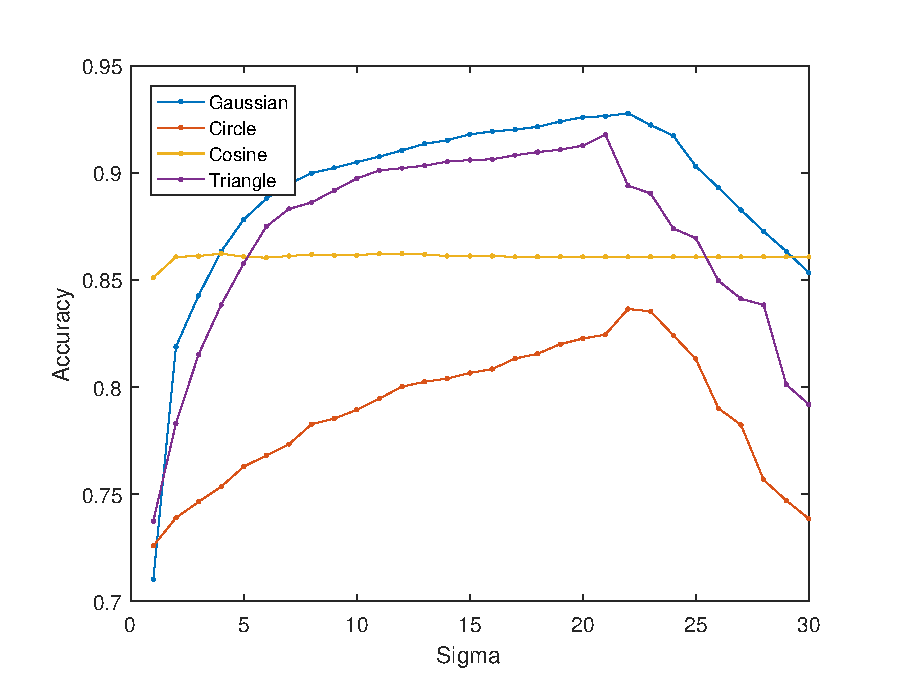
\includegraphics[width=0.5\textwidth,height=1.6in]{sigma.eps}
    \setlength{\abovecaptionskip}{-0.1cm}
    \caption{For different kernel functions, the relationship between sentiment analysis accuracy and $\sigma$}\label{fig:sigma}
\end{figure}

Among the four kernel functions, the Cosine kernel function is less affected by sigma. The accuracy of sentiment extraction corresponding to the other three kernel functions increases first and then decreases, and all three kernel functions get the optimal value when the value of sigma is approximately equal to 21. The Gaussian kernel function performs best. So we take the Gaussian kernel function as a form of the distance function and set the value of sigma to 21. Under such conditions, the sentiment extraction accuracy of the data set reached 92.77 percent.



\subsection{Evaluation of Public Opinion Model}
Here, we show the advantages of our model in simulating the evolution of public opinion. 

Parameter $\alpha$ represents the distribution of background opinion in the incidents. As shown in Fig~\ref{fig:alpha}, the $\alpha$ is smoothly and slowly changing in all six incidents as we considered before. The $\alpha$ of WZXHospital, RYBabused, CFfall, and SDhumiliation is less than 0.5, indicating that negative sentiment is the public’s backgronund opinion to these incidents. The $\alpha$ of JGmurder and HZbabysitter are greater than 0.5, indicating that positive sentiment is the public’s backgronund opinion to these incidents.

\vspace{-0.6cm}
\begin{figure}
\centering
\subfigure[CFfall]{\label{fig:time0}
    \centering
    \includegraphics[width =.3\textwidth]{cfzla.eps}
}
\hspace{-0.15cm}
\subfigure[RYBabused]{\label{fig:hhl}
    \centering
    \includegraphics[width =.3\textwidth]{hhl.eps}
}
\hspace{-0.15cm}
\subfigure[HZbabysitter]{\label{fig:hzbml}
    \centering
    \includegraphics[width =.3\textwidth]{hzbm.eps}
}
\vspace{-0.3cm}
\subfigure[JGmurder]{\label{fig:jg}
    \centering
    \includegraphics[width =.3\textwidth]{jg.eps}
}
\hspace{-0.15cm}
\subfigure[SDhumiliation]{\label{fig:sdrma}
    \centering
    \includegraphics[width =.3\textwidth]{sdrma.eps}
}
\hspace{-0.15cm}
\subfigure[WZXHospitaln]{\label{fig:wzx}
    \centering
    \includegraphics[width =.3\textwidth]{wzx.eps}
}
\caption{Changes in the $\alpha$ value of six events}\label{fig:alpha}
\end{figure}

We choose precision and recall as evaluation metrics to evaluate the performance of finding shift points. We compare our model with POMS, FB-LDA and RCB-LDA. POMS use the sentiment extraction tool to measure the sentiment polarity at numerous time points and use residual to extract shift points. FB-LDA and RCB-LDA are topic-based methods. The ground truth of shift points are manually determined. We have five people voting for Whether each time point of the six incidents belongs to the shift point. 
\begin{figure}
\centering
\subfigure[Precision]{\label{fig:precision}
    \centering
    \includegraphics[width =.4\textwidth]{precision.eps}
}
\hspace{-4ex}
\subfigure[Recall]{\label{fig:recall}
    \centering
    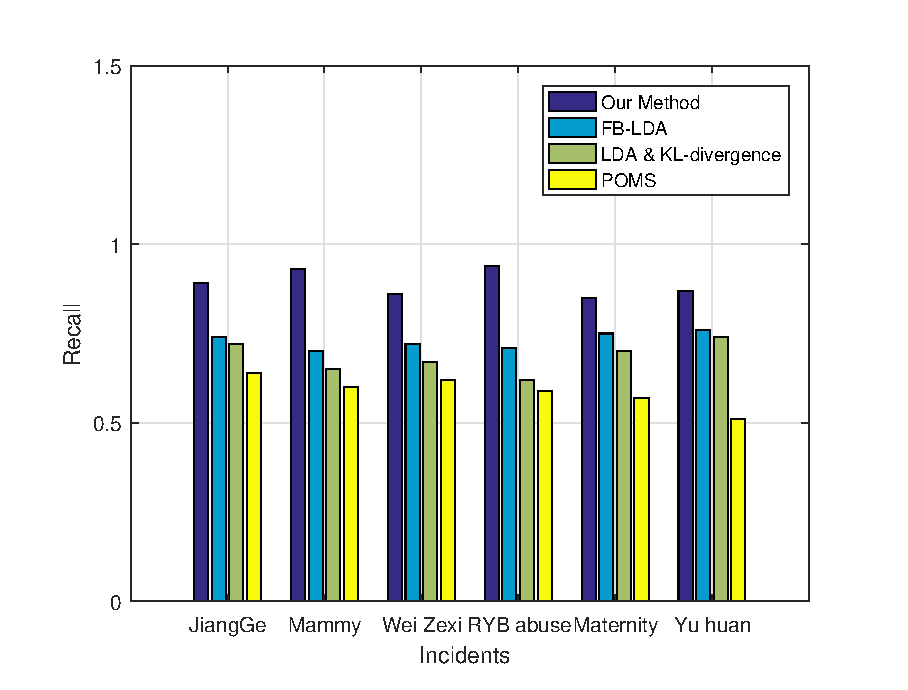
\includegraphics[width =.4\textwidth]{recall.eps}
}
\setlength{\abovecaptionskip}{-0.1cm}
\caption{Comparative preformance of shift detection}\label{fig:shift}
\end{figure}

As shown in Fig~\ref{fig:shift}, Our model has achieved the best results in detecting shift points. For the six events we selected, our model can achieve an average of 86\% precision and 90\% recall. In contrast, the average precision and recall of FB-LDA are 81\% and 73\%. For RCB-LDA are 76\% and 68\%. POMS performs the worst which the average precision and recall are 52\% and 59\%. These results show that our model can accurately detect the punblic opinion shift in the incident.

\vspace{-0.5cm}
\begin{figure}
    \centering
    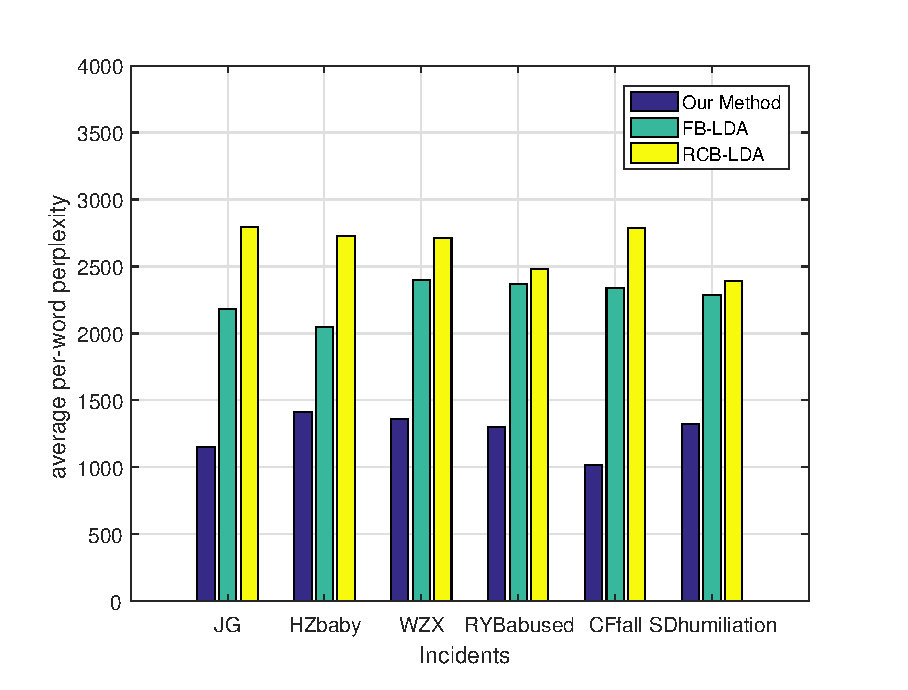
\includegraphics[width=0.5\textwidth,height=1.6in]{perplexity.eps}
    \setlength{\abovecaptionskip}{-0.1cm}
    \caption{Averaged per-word predictive perplexity comparison}\label{fig:perplexity}
\end{figure}

We evaluated the model predictive performance with perplexity which is a evaluation standard for measuring the predictive performance of a model. For each incident, We compute the averaged per-word perplexity over the time line of our model, FB-LDA and RCB-LDA. As shown in Fig~\ref{fig:perplexity},  Compared to the other two methods, our model has a smaller averaged per-word perplexity in all six incidents. This result indicates our model has better predictive performance.







\section{Conclusion}\label{sec:conclusion}
In this paper, we study the problem of tracking the evolution of public opinion in social events. We analyze the differences between social events and entities in sentiment analysis, and propose a new opinion evolution model to track the changes in public opinion in social events. We consider the existence of background opinion distribution in the model, and use probability to indicate the likelihood of sudden changes in sentiments at each time point. To improve the performance of our model, we add entities in the process of sentiment analysis, use the distance function to calculate the influence of emotional words on entities, and experimentally prove that the distance function is more effective for long comments. In the future, we plan to track changes in public opinion about different entities in social events. Changes in opinions of different entities can reflect the relationship between entities.
\begin{thebibliography}{8}

\bibitem{Cheung2014Battle}
Cheung A S Y. 
\newblock The Battle of Microblogging for Legal Justice in China. 
\newblock Ssrn Electronic Journal, 2014.

\bibitem{Giachanou2016sentichange}
Anastasia Giachanou, Ida Mele and Fabio Crestani.
\newblock  Explaining Sentiment Spikes in Twitter.
\newblock In CIKM ’16, PP. 2263-2268, 2016.

\bibitem{Giachanou2017sentichange}
Anastasia Giachanou, Ida Mele and Fabio Crestani.
\newblock  A Collection for Detecting Triggers of Sentiment Spikes.
\newblock In SIGIR ’17, PP. 1249-1252, 2017.

\bibitem{Tsytsarau2014Topics}
Mikalai Tsytsarau, Themis Palpanas and Malu Castellanos.
\newblock  Dynamics of news events and social media reaction.
\newblock In KDD ’14, PP. 901-910, 2014.

\bibitem{Thelwall2011topic}
Mike Thelwall, Kevan Buckley, and Georgios Paltoglou.
\newblock Sentiment in Twitter Events.
\newblock In Journal, pp. 406-418, 2011.

\bibitem{sentistrength2010}
Mike Thelwall, Kevan Buckley, Georgios Paltoglou, Di Cai, and Arvid Kappas.
\newblock Sentiment strength detection in short informal text.
\newblock Journal of the Association for Information Science and Technology 61, 12 (2010), 2544–2558.

\bibitem{Thelwall2012lexicon}
Mike Thelwall, Kevan Buckley, and Georgios Paltoglou. 2012.
\newblock Sentiment strength detection for the social web.
\newblock J. Am. Soc. Inform. Sci. Technol. 63, 1 (2012), 163–173.

\bibitem{Ortega2013lexicon}
Reynier Ortega, Adrian Fonseca, and Andres Montoyo. 2013.
\newblock SSA-UO: Unsupervised twitter sentiment analysis.
\newblock In Proceedings of the 7th International Workshop on Semantic Evaluation.

\bibitem{Giachanou2016sentitime}
Anastasia Giachanou, Fabio Crestani. 2011.
\newblock Tracking Sentiment by Time Series Analysis.
\newblock In SIGIR ’16, pp. 1037-1040, 2016

\bibitem{An2014sentimentchange}
X. An, R. A. Ganguly, Y. Fang, B. S. Scyphers, M. A. Hunter, and G. J.
\newblock Tracking Climate Change Opinions from Twitter Data. 
\newblock In KDD’14: Workshop on Data Science for Social Good, 2014.

\bibitem{Bollen2011sentimentchange}
J. Bollen, A. Pepe, and H. Mao.
\newblock Modeling Public Mood and Emotion : Twitter Sentiment and Socio-Economic Phenomena. 
\newblock In ICWSM’11, pages 450-453, 2011.

\bibitem{Tan2014topic}
Shulong Tan, Yang Li, Huan Sun, Ziyu Guan.
\newblock Interpreting the Public Sentiment Variations on Twitter. 
\newblock In Journal’14, 2014.

\bibitem{Montero2016sentimentchange}
C. S. Montero, H. Haddad, M. Mozgovoy, and C. B. Ali.
\newblock Detecting the likely causes behind the emotion spikes of influential twitter users. 
\newblock In CICLing’16, 2016.

\bibitem{Ahmed2017SentiCR}
Toufique Ahmed, Amiangshu Bosu, Anindya Iqbal, Shahram Rahimi.
\newblock SentiCR: A Customized Sentiment Analysis Tool for Code Review Interactions.
\newblock In ASE ’17, 2017.

\bibitem{Go2009Supervisedlearning}
Alec Go, Richa Bhayani, and Lei Huang. 2009.
\newblock Twitter Sentiment Classification Using Distant Supervision.
\newblock Technical Report. Standford.

\bibitem{Barbosa2010Supervisedlearning}
Luciano Barbosa and Junlan Feng.2010.
\newblock Robust sentiment detection on twitter from biased and noisy data.
\newblock In COLING ’10, pp. 36-44, 2010.

\bibitem{Papadopoulos2012SocialEvent}
Efthymios Kouloumpis, Theresa Wilson, and Johanna Moore. 2011.
\newblock Twitter sentiment analysis: The good the bad and the omg!
\newblock In ICWSM’11, pp. 538-541.

\bibitem{Pak2010Supervisedlearning}
Alexander Pak and Patrick Paroubek. 2010.
\newblock Twitter as a corpus for sentiment analysis and opinion mining.
\newblock In LREC ’10, pp. 1320-1326, 2010.

\bibitem{Davidov2010Supervisedlearning}
Dmitry Davidov, Oren Tsur, and Ari Rappoport.2010.
\newblock Enhanced sentiment learning using twitter hashtags and smileys.
\newblock In COLING ’10, pp. 241-249, 2010.

\bibitem{Agarwal2010Supervisedlearning}
Apoorv Agarwal, Boyi Xie, Ilia Vovsha, Owen Rambow, and Rebecca Passonneau. 2010.
\newblock Sentiment analysis of twitter data.
\newblock In LCM’11, pp. 30–38.

\bibitem{Hutto2014SSimproved}
C. J. Hutto and E. Gilbert. 2014.
\newblock Vader: A parsimonious rule-based model for sentiment analysis of social media text.
\newblock In AAAI’14.

\bibitem{Rakibul2017SentiStrength-SE}
Md Rakibul Islam and Minhaz F Zibran. 2017.
\newblock Leveraging automated sentiment analysis in software engineering. 
\newblock In Proceedings of the 14th International Conference on Mining Software Repositories. IEEE Press, 203-214.

\bibitem{Feng2011lexicon}
Song Feng, Ritwik Bose, and Yejin Choi. 2011.
\newblock Learning general connotation of words using graph-based algorithms.
\newblock In EMNLP ’11, pp. 1092-1103, 2011.

\bibitem{Zhang2012corenodes}
Tiantian Zhang, Bin Wu.
\newblock A Method for Local Community Detection by Finding Core Nodes. 
\newblock In Proceedings of the 2012 IEEE/ACM International Conference on Advances in Social Networks Analysis and Mining.




\end{thebibliography}


\end{document}



